\documentclass[tikz,border=2pt]{standalone}
\usepackage{amsmath}
\usepackage{pgfplots}
\pgfplotsset{compat=1.18}
\begin{document}
% x'(t) = 3x(t): short grey segments of slope 3x show the prescribed rate at each state; the
% solutions x(t) = Ce^{3t} (C = -2, -1, 0, 1, 3) follow them, and x(0) = 2 picks C = 2.
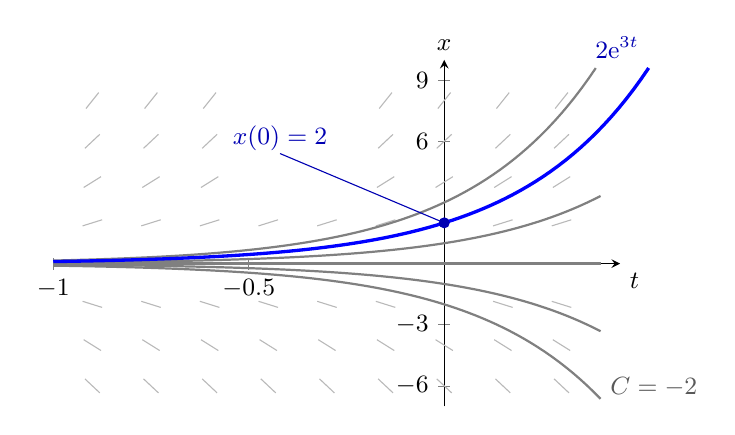
\begin{tikzpicture}[font=\small]
  \begin{axis}[
    axis lines=middle, xmin=-1, xmax=0.45, ymin=-7, ymax=10,
    xtick={-1,-0.5}, ytick={-6,-3,6,9},
    xlabel={$t$}, ylabel={$x$}, xlabel style={anchor=north west}, ylabel style={anchor=south},
    scale only axis, width=7.2cm, height=4.4cm, clip=false, samples=80
    ]
    % slope field: segments of display length 0.26 cm and slope 3x (1 unit = 4.97 cm in t, 0.259 cm in x)
    \foreach \t in {-0.9,-0.75,...,0.31} {
      \foreach \x in {-6,-4,...,8} {
        \pgfmathsetmacro{\n}{sqrt(4.97^2+(0.259*3*\x)^2)}
        \pgfmathsetmacro{\du}{0.13/\n}
        \pgfmathsetmacro{\dv}{0.13*3*\x/\n}
        \pgfmathtruncatemacro{\keep}{(\t<-0.5)||(\t>-0.2)||(\x<4)}% leave room for the label
        \ifnum\keep=1
          \edef\seg{\noexpand\draw[gray!55] (axis cs:\t-\du,\x-\dv) -- (axis cs:\t+\du,\x+\dv);}
          \seg
        \fi
      }
    }
    \foreach \c in {-2,-1,0,1,3} {
      \edef\curve{\noexpand\addplot[gray, thick, domain=-1:{min(0.4,ln(9.6/abs(\c+0.001))/3)}] {\c*exp(3*x)};}
      \curve
    }
    \addplot[blue, very thick, domain=-1:{ln(4.8)/3}] {2*exp(3*x)};
    \fill[blue!70!black] (axis cs:0,2) circle (2pt);
    \draw[blue!70!black, thin] (axis cs:0,2) -- (axis cs:-0.42,5.4);
    \node[blue!70!black, anchor=south, inner sep=1pt] at (axis cs:-0.42,5.4) {$x(0)=2$};
    \node[blue!70!black, anchor=south east] at (axis cs:{ln(4.8)/3},9.6) {$2\mathrm{e}^{3t}$};
    \node[gray!70!black, anchor=west] at (axis cs:0.4,{-2*exp(1.2)+0.6}) {$C=-2$};
  \end{axis}
\end{tikzpicture}
\end{document}
